\chapter[Projeto de Energia]{Projeto de Energia}

\section{Objetivo Específico}

Analisar o sistema de arrefecimento (transferências de calor), sistema de admissão (fluxo de ar), sistema de exaustão (emissões gasosas), consumo de combustível e desempenho de um motor a combustão interna por meio de um ensaio a vazio.

\section{Concepção e detalhamento do subsistema}

Devido ao fator de integração do projeto (funcionamento do motor, sensoriamento e leitura de dados), não foi possível a obtenção de análises para o Ponto de Controle 2. Ressaltando que toda instrumentação necessária já está disponível.

\subsection{Sistema de Arrefecimento}

A temperatura do motor de combustão interna (MCI) influencia no consumo de combustível, na eficiência e na emissão de gases, portanto este é um importante parâmetro a ser avaliado nos testes dos motores \cite{kuntzer15}.

A transferência de energia de calor no motor ocorre por condução, convecção e por radiação. Os trocadores de calor são os principais dispositivos que irão propiciar esta transferência de calor para o ambiente. O radiador é um tipo de trocador de calor que são geralmente classificados como compactos e de escoamento cruzado sem mistura.

O trocador de calor utilizado no laboratório de testes do MCI é o modelo 7351123R da Valeo, Figura \ref{radiador}:

\begin{figure}[h!]
	\centering
	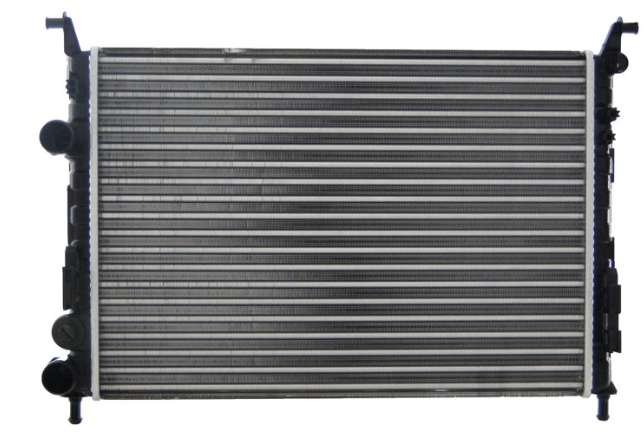
\includegraphics[keepaspectratio=true,scale= 0.35]{figuras/radiador.png}
	\caption{Radiador utilizado no laboratório de testes de MCI. Fonte: APS Distribuidora.}
	\label{radiador}
\end{figure}

As dimensões são mostradas na Figura \ref{dimensoes-radiador} a seguir:

\begin{figure}[h!]
	\centering
	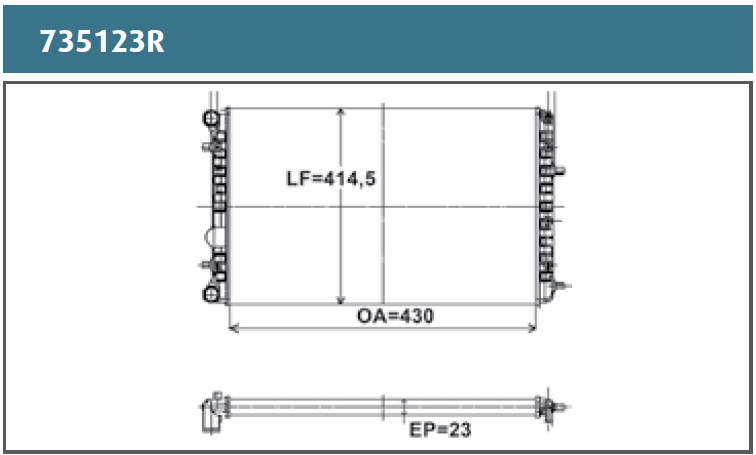
\includegraphics[keepaspectratio=true,scale= 0.4]{figuras/dimensoes-radiador.png}
	\caption{Dimensões do radiador. Fonte: Catálogo Valeo Arrefecimento.}
	\label{dimensoes-radiador}
\end{figure}

Admitindo-se que o escoamento é permanente, a taxa de transferência de calor do fluido quente será igual a taxa de transferência de calor do fluido frio e pode ser determinada por \cite{energiaTransferencia}:

\begin{equation}
	Q = mc_{ph}(T_{h, in} - T_{h, out}) = mc_{pc}(T_{c, in} - T_{c, out})
\end{equation}

Utilizando o método da diferença de temperatura média logarítmica (LMTD) e conhecendo-se as temperaturas na entrada e na saída, a taxa de transferência de calor também poderá ser definida por \cite{energiaTransferencia}:

\begin{equation}
	Q = UA_{s}\Delta T_{lm}
\end{equation}

Onde:

$Q$: taxa transferência de calor;

$U$: coeficiente global de transferência de calor;

$A_{s}$: área de superfície;

$\Delta T_{lm}$: diferença de temperatura média logarítmica.

A diferença de temperatura média logarítmica é dada por :

\begin{equation}
	\Delta T_{lm} = \frac{\Delta T_{1}-\Delta T_{2}}{ln \frac{\Delta T_{1}}{\Delta T_{2}}}
\end{equation}

$\Delta T_{1}$ e $\Delta T_{2}$ são as diferenças de temperatura entre os dois fluidos.

Para o trocador de calor de escoamento cruzado em que os fluidos não se misturam utiliza-se um fator de correção F que pode ser encontrado no gráfico da Figura \ref{fator-de-correcao}:

\begin{figure}[h!]
	\centering
	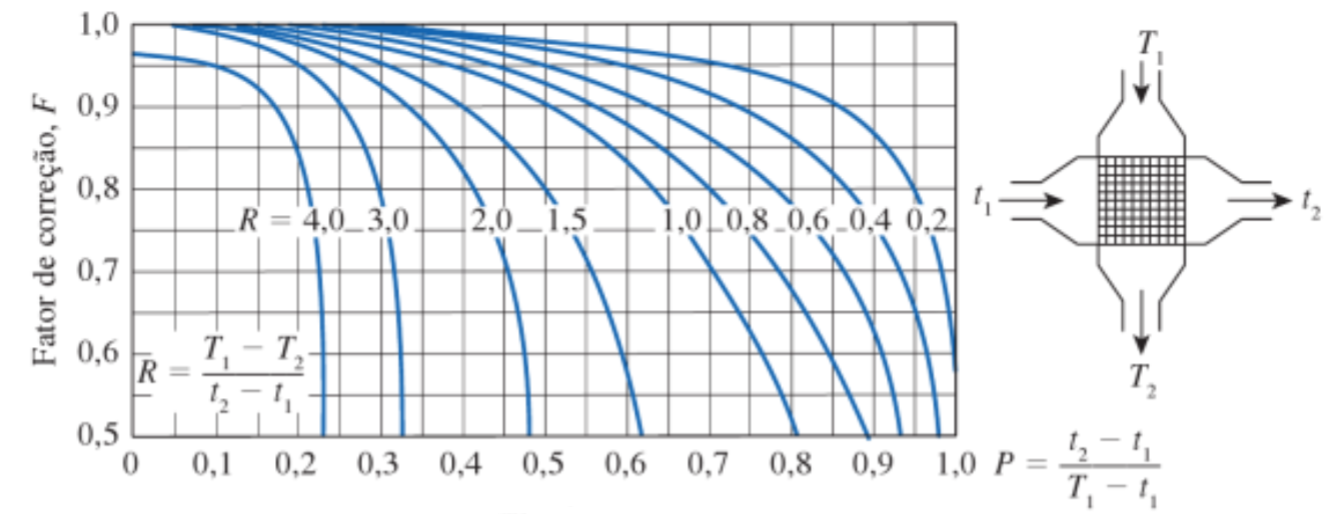
\includegraphics[keepaspectratio=true,scale= 0.3]{figuras/fator-de-correcao.png}
	\caption{Fator de correção para trocador de calor de único passe e com fluidos sem mistura.\cite{energiaTransferencia}}
	\label{fator-de-correcao}
\end{figure}

Sendo que o trocador de calor já está definido, busca-se a determinação da efetividade de tal trocador. Para isso é utilizado o método da efetividade-NTU. A efetividade do trocador de calor é definida como se segue \cite{energiaTransferencia}:

\begin{equation}
	\varepsilon = \frac{Q}{Q_{max}} = \frac{taxa\,de\,transferência\,de\,calor\,real}{taxa\,de\,transferência\,de\,calor\,máxima}
\end{equation}

A taxa de transferência de calor máxima é determinada por:

\begin{equation}
	Q_{max} = C_{min} (T_{h, in} - T_{h, out})
\end{equation}

Onde $C_{min}$ é a taxa de capacidade térmica do fluido de menor capacidade térmica e é dada pela seguinte equação:

\begin{equation}
	C_{min} = mc_{p}
\end{equation}

O número de unidades de transferência de calor, NTU, é:

\begin{equation}
	NTU = \frac{UA_{s}}{C_{min}}
\end{equation}

A efetividade do radiador poderá ser definida pela seguinte equação:

\begin{equation}
	\varepsilon = 1 - e^{\left [ \left ( \frac{C_{min}}{C_{max}} \right ) ^{-1} \left ( NTU \right ) ^{0,22} \left \{ e^{\frac{-C_{min}}{C_{max}} \left ( NTU \right ) ^{0,22}} -1 \right \} \right ]}
\end{equation}

Os sensores de temperatura serão posicionados na mangueira do radiador antes da entrada do fluido de arrefecimento no bloco do motor e depois de ter sido feito o resfriamento do motor, ou seja, na saída do motor. Sendo assim, será possível ter o controle da temperatura no motor e fazer as avaliações de troca de calor.

Para fazer os cálculos da transferência de calor, é necessário conhecer os parâmetros de fluxo de água na mangueira do radiador e o fluxo de ar pelo radiador. A medida do fluxo de água será feita por meio de um sensor medidor de fluxo e a medida do fluxo de ar será feita medindo-se a velocidade do fluxo de ar através do núcleo do radiador com o auxílio de um anemômetro e assim, calcula-se a vazão de ar multiplicando a velocidade pela área frontal do radiador.

O calor rejeitado do motor é proporcional à potência útil, portanto deverá ser gerado um gráfico do calor gerado a diferentes rotações do motor.

\subsection{Sistema de Admissão}

A caixa estabilizadora de orifício calibrado permite que o ar que entra na admissão do motor tenha tenha uma vazão constante.

Os dados do plenum que serão coletados pelos sensores são os valores de pressão e temperatura. Estes serão utilizados para o cálculo da vazão mássica de ar que será empregada para o cálculo da razão ar/combustível.

Considere o esquema de admissão da Figura \ref{esquema-de-admissao}, a seguir:

\begin{figure}[h!]
	\centering
	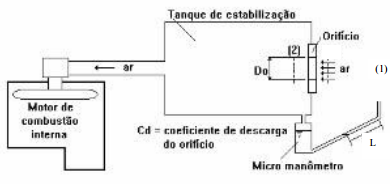
\includegraphics[keepaspectratio=true,scale= 0.8]{figuras/esquema-de-admissao.png}
	\caption{Esquema de Admissão.}
	\label{esquema-de-admissao}
\end{figure}

Aplicando a equação de Bernoulli entre os pontos 1 e 2 tem-se:

\begin{equation}
	\frac{v_{1}^{2}}{2_{g}} + \frac{P_{1}}{\gamma _{ar}} + Z_{1} = \frac{v_{2}^{2}}{2_{g}} + \frac{P_{2}}{\gamma _{ar}} + Z_{2}
\end{equation}

\begin{equation}
	\gamma _{ar} = \rho g = cte
\end{equation}

\begin{equation}
	P_{1} - P_{2} = h\gamma _{H20}
\end{equation}

\begin{equation}
	h = Lsen\theta
\end{equation}

\begin{equation}
	v_{2} = \sqrt{\frac{2gh\gamma _{h20}}{\gamma _{ar}}}
\end{equation}

A vazão teórica é:

\begin{equation}
	Q_{t} = \frac{\pi D_{0}^{2}}{4}\sqrt{\frac{2gh\gamma _{h20}}{\gamma _{ar}}}
\end{equation}

E a vazão real:

\begin{equation}
	Q_{r} = C_{d,o}Q_{t}
\end{equation}

A vazão mássica do ar é:

\begin{equation}
	m_{ar} = \rho _{ar}Q_{r}
\end{equation}

Essa é a vazão mássica de ar realmente admitida pelo motor  e que será utilizada para o cálculo da razão ar/combustível consumida.

\subsection{Instalação do Dinamômetro}

O conjunto de equipamentos do dinamômetro presente no laboratório de testes do motor de combustão interna é composto por uma central de comando, um motor, um sistema de refrigeração acoplado ao motor e um banco de baterias.

Devido ao fato do conjunto estar na universidade por cerca de 7 anos sem utilização, a principal ação necessária seria a identificação do tipo de motor para a realização dos testes de manutenção específicos para avaliação das condições de funcionamento da máquina.

No entanto, um entrave encontrado para a realização dos testes foi a não caracterização da máquina devido a falta de informação nas placas de identificação.

Sendo assim, descartou-se a utilização do dinamômetro na bancada de testes devido a limitação de informações e ao tempo que limita a realização do trabalho.


\subsection{Análise de Emissões}

A maior fonte de poluição urbana do ar pode ser relacionado com o motor a combustão interna, pois além do gás carbônico produzido nas reações de combustão, outros gases também são formados, como  o monóxido de carbono ($CO$), óxidos de nitrogênio ($NO_{x}$), hidrocarbonetos ($HC$), oxigênio ($O_{2}$), compostos orgânicos voláteis (COVs), entres outros.

O órgão que delimita os limites legais de emissões veiculares, no Brasil, é o Conselho Nacional do Meio Ambiente (CONAMA). Para a implementação das resoluções, o CONAMA criou o Programa de Controle da Poluição do Ar por Veículos Automotores (PROCONVE) para os veículos leves e pesados, fixando prazos, limites máximos de emissões e estabelecendo exigências tecnológicas para veículos automotores, nacionais e importados \cite{energiaAvaliacao}.

Ao conhecer os mecanismos de formação de poluentes gerados pelo motor, pode-se associar a tecnologias de gerenciamento de controle. Com isso, compreende-se que os níveis de emissões gasosas veiculares podem ser controlados e regulamentados, adequando-se aos padrões exigidos pela legislação e buscando uma menor poluição do meio ambiente.

Na bancada de teste do MCI, esta medição será feita por meio do analisador de gases universal (PC-MULTIGÁS) baseado no método de medição de infravermelho não dispersivo.

\begin{table}[h!]
\centering
\caption{Dados técnicos do analisador de gases \cite{napro}.}
\label{my-label}
\begin{tabular}{|c|c|}
\hline
\textbf{ALIMENTAÇÃO}        & 12VDC ou 110/110AVC – 60Hz                                                                                    \\ \hline
\textbf{ESCALAS}            & \begin{tabular}[c]{@{}c@{}}CO: 0 - 15\%\\ CO2: 0 - 20\%\\ HC: 0 - 20000ppm Hexano\\ O2: 0 - 25\%\end{tabular} \\ \hline
\textbf{DIMENSÕES} & 290 x 150 x 310 mm                                                                                            \\ \hline
\textbf{PESO}               & 4 Kg                                                                                                          \\ \hline
\end{tabular}
\end{table}

O equipamento será acoplado ao coletor do motor (sistema de exaustão) por meio de uma mangueira contendo na extremidade de contato uma sonda de captação de gases. Assim as medições ($CO$, $CO_{2}$, $HC$ e $O_{2}$) serão coletadas pelo analisador e enviadas para o scanner PC-SCAN que mostrará o diagnóstico veicular.

\begin{figure}[h!]
	\centering
	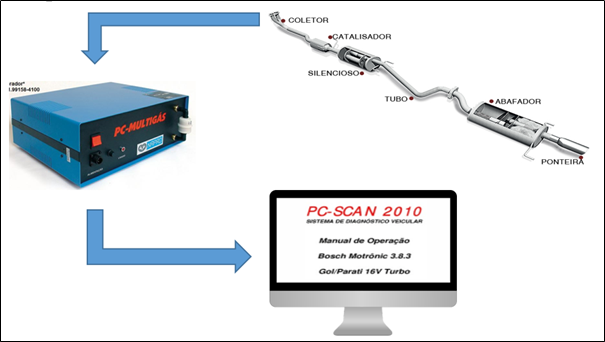
\includegraphics[keepaspectratio=true,scale= 1.0]{figuras/esquematico-operacional.png}
	\caption{Esquemático operacional para análise de emissões.}
	\label{esquematico-operacional}
\end{figure}

O método usado pelo equipamento para obtenção dos dados utiliza o princípio de que as moléculas de um determinado gás absorvem o raio infravermelho e analisa de forma contínua a variação da concentração de um componente específico de uma mistura gasosa, sendo denominado como método de medição de infravermelho não dispersivo \cite{nereu}.

Basicamente, cada componente (molécula), possui um comprimento de onda (e frequência correspondente) específico, baseado nisso e na transmitância, é possível obter a concentração de determinados componentes que estão situados na região IR ($infrared$).

A partir dos dados obtidos pelo programa, será feita uma análise relacionando as porcentagens de cada gás emitido com a composição do combustível utilizado. Observando também toda questão legislativa mencionada anteriormente, pois é um fator imprescindível para a indústria automotiva.

\subsection{Consumo de combustível}

Tendo como análise um motor a gasolina, os ensaios serão realizados utilizando três misturas:

\begin{itemize}
\item Gasolina pura;
\item Gasolina Comum Brasileira (tipo C): mistura E27 - correspondente a um percentual de 73\% de gasolina pura e 27\% de álcool anidro (AEAC);
\item Mistura E50: correspondente a um percentual de 50\% de gasolina pura e 50\% de álcool anidro (AEAC);
\end{itemize}

Para obtenção da gasolina com máximo grau de pureza, foi utilizado o método de extração líquido-líquido. Sendo baseado na diferença de solubilidade do álcool na gasolina e na solução de $NaCl$ (usada para aumentar a solubilidade do álcool em água, pois sendo este sal um composto iônico, a sua solução é mais polar do que a água pura, desta maneira consegue-se extrair com mais eficiência o álcool da camada orgânica, gasolina).

Quanto a medição do consumo de combustível foi considerado o método mássico que consiste em colocar uma balança sob o tanque de combustível. Utilizando-se da escala da balança como referência, quando o ponteiro passar por um valor conhecido aciona-se o cronômetro e quando o ponteiro passar por um novo valor conhecido, para-se o cronômetro \cite{taylor}.

\begin{figure}[h!]
	\centering
	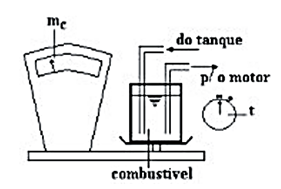
\includegraphics[keepaspectratio=true,scale= 0.6]{figuras/medicao-de-consumo.png}
	\caption{Método mássico de medição de consumo.}
	\label{medicao-de-consumo}
\end{figure}

 O acionamento e desligamento do cronômetro será feito por um sensor de infravermelho. Tendo assim uma massa consumida em um determinado tempo ($t$), o que é exatamente a vazão em massa de combustível consumido. A partir disso será feito um conjunto de análises, como: gráfico de consumo de combustível por velocidade angular ($rpm$); emissões geradas e desempenho do motor.

\begin{figure}[h!]
	\centering
	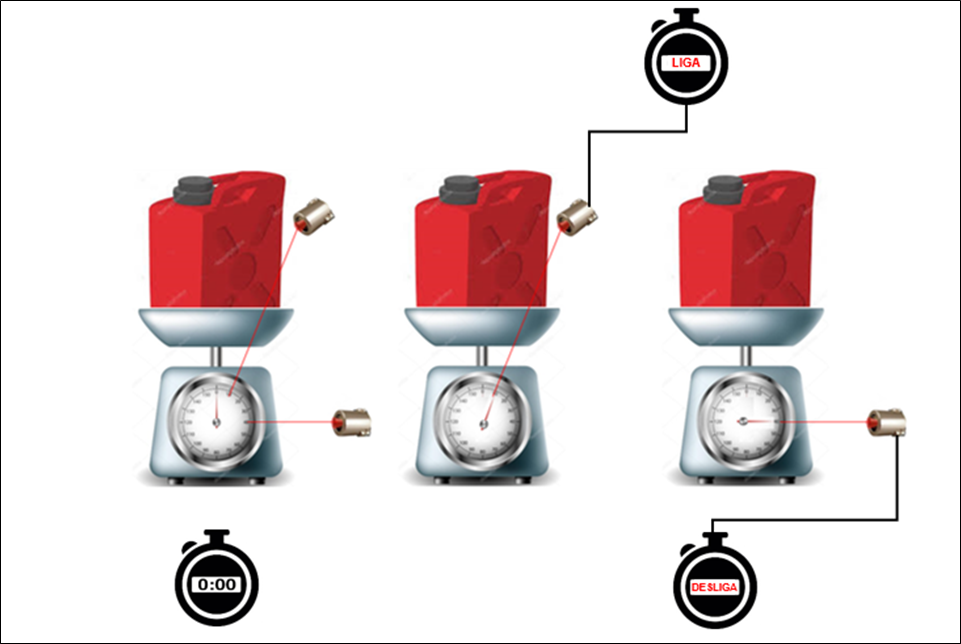
\includegraphics[keepaspectratio=true,scale= 0.6]{figuras/funcionamento-cronometro.png}
	\caption{Funcionamento do cronômetro a partir dos sensores de infravermelho.}
	\label{funcionamento-cronometro}
\end{figure}